\clearpage
\chapter{Reading and Writing Notation}

\classquote{不积跬步，无以至千里；不积小流，无以成江海。\\
Without accumulating single steps, one cannot reach a thousand li; without accumulating small streams, one cannot form rivers and seas.}{Xunzi · Encouraging Learning}{There is no shortcut to reading notation: learn one bar’s pitches and durations each day, and the page slowly turns into movement in your hands. Accuracy first, speed second; translate the page into the piano roll before you try to sight-read.}

\label{sec:reading-notation}

\section*{What you can do after this chapter}
\begin{itemize}
  \item Read a staff's clef, time signature, and key signature, and name the pitch on a given line or space.
  \item Convert common notes, rests, dots, and ties into beats and durations instead of guessing from the shape.
  \item Recognise dynamics, tempo, and common expression marks and know roughly what they ask a performer to do.
  \item Translate a simple score into note names, MIDI numbers, and piano-roll rows, then enter it in Yeban by hand.
\end{itemize}

\section{The staff: lines and spaces are not decoration}

A staff has five parallel horizontal lines. The gaps between them are called spaces. From the bottom up, the five lines and four spaces each represent one diatonic step; neighbouring lines or spaces differ by a natural step, not by a fixed two semitones. The clef fixes which pitch that set of positions starts from, so the same line means a completely different note in treble and bass clefs.

The treble clef is the most common. Its five lines, from bottom to top, are E4, G4, B4, D5, and F5; its four spaces are F4, A4, C5, and E5. A simple memory aid is ``E G B D F'' bottom to top, with spaces ``F A C E.'' Middle C (C4) is not inside the five lines; it sits on a short ledger line below the treble staff. D4 is in the space above middle C, and E4 returns to the first line.

The bass clef's five lines, bottom to top, are G2, B2, D3, F3, and A3; its four spaces are A2, C3, E3, and G3. Middle C is on the first ledger line above the bass staff. A grand staff places treble and bass staves one above the other, with middle C between them; when reading a grand staff, first see which staff the note belongs to, then use that clef.

\begin{center}
\begin{minipage}{0.96\linewidth}
\centering
\begin{tikzpicture}[x=1cm,y=1cm,font=\scriptsize]
  \foreach \y in {0,1,2,3,4} {\draw[gray] (0,\y) -- (10,\y);}
  \draw[gray] (0,-1) -- (10,-1);
  \node[left,font=\tiny] at (0,4) {fifth line};
  \node[left,font=\tiny] at (0,0) {first line};
  \node[left,font=\tiny] at (0,-1) {ledger};
  \node[below,font=\tiny] at (0.3,-1.55) {treble clef};
  \foreach \x/\y/\n in {1.2/-1/C4,2.4/-0.5/D4,3.6/0/E4,4.8/0.5/F4,6.0/1/G4,7.2/1.5/A4,8.4/2/B4,9.3/2.5/C5} {
    \fill (\x,\y) ellipse (0.10 and 0.07);
    \node[above=1pt,font=\tiny] at (\x,\y) {\n};
  }
\end{tikzpicture}

Figure 9-1: treble-clef lines and spaces, with middle C on its ledger line. Adjacent lines/spaces are one diatonic step; E--F and B--C are only a semitone apart, while the other adjacent steps are two semitones.
\end{minipage}
\end{center}

Do not read by counting every line from the first note. Find anchors first: middle C, first-line E4, and third-line B4 in treble clef; middle C, first-line G2, and third-line D3 in bass clef. Once the anchors are fixed, other notes are nearby lines and spaces, which is much faster.

\section{Notes, rests, and durations}

A note's shape shows duration, not pitch. A whole note is a hollow oval; a half note adds a stem; a quarter note is filled and has a stem; an eighth note adds one flag; a sixteenth adds two flags. More flags mean a shorter value; each extra flag halves the duration.

In 4/4, a whole note lasts four beats, a half note two, a quarter note one, an eighth note half a beat, and a sixteenth a quarter of a beat. A dot lengthens a note by half its value: a dotted half is three beats, a dotted quarter is one and a half beats. A tie joins adjacent notes of the same pitch into one longer sound without re-attacking; ties across bar lines are the most common.

A rest means ``no sound here,'' with durations matching the note names: whole rest, half rest, quarter rest, eighth rest, sixteenth rest. A rest is not a missing note; it is part of the rhythm. Music with no rests feels constantly pressed and lacks breathing room.

\begin{center}
\begin{minipage}{0.94\linewidth}
\centering
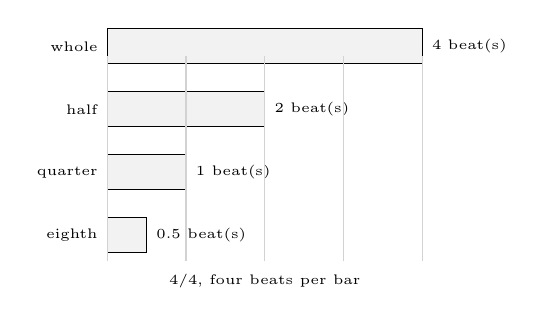
\begin{tikzpicture}[x=1cm,y=1cm,font=\scriptsize]
  \foreach \r/\lab/\w in {0/whole/4,1/half/2,2/quarter/1,3/eighth/0.5} {
    \draw[fill=gray!10] (0,-\r*0.8) rectangle ++(\w,0.45);
    \node[left,font=\tiny] at (0,-\r*0.8+0.22) {\lab};
    \node[right,font=\tiny] at (\w,-\r*0.8+0.22) {\w{} beat(s)};
  }
  \foreach \x in {0,1,2,3,4} {\draw[gray!35] (\x,0.1) -- (\x,-2.5);}
  \node[below,font=\tiny] at (2,-2.55) {4/4, four beats per bar};
\end{tikzpicture}

Figure 9-2: proportional lengths of four common values in 4/4. Length follows beat count, not the visual size of the notehead.
\end{minipage}
\end{center}

\begin{center}
\small
\begin{tabular}{p{0.16\linewidth}p{0.18\linewidth}p{0.16\linewidth}p{0.32\linewidth}}
\toprule
Note & Beats in 4/4 & Rest & Remark \\
\midrule
Whole & 4 & Whole rest & The basic unit of a bar \\
Half & 2 & Half rest & Two halves fill a bar \\
Quarter & 1 & Quarter rest & The most common beat unit \\
Eighth & 0.5 & Eighth rest & Two eighths equal one quarter \\
Sixteenth & 0.25 & Sixteenth rest & Four sixteenths equal one quarter \\
Dotted quarter & 1.5 & --- & Adds half; often paired with an eighth \\
\bottomrule
\end{tabular}

Table 9-1: common notes, rests, and their values in 4/4. Dots and ties change the sounding length; count them separately when reading.
\end{center}

A time signature sits at the start of the staff: the top number is beats per bar, the bottom number is the beat unit. 4/4 means four beats per bar with the quarter note as one beat; 6/8 means six beats per bar with the eighth note as one beat. The time signature is not tempo; tempo comes from BPM or a tempo mark. 120 BPM in 4/4 means 120 quarter notes per minute; 120 BPM in 6/8 means 120 eighth notes per minute.

\section{Key signatures, dynamics, and expression}

A key signature sits beside the time signature and uses sharps or flats to tell you which notes are raised or lowered. One sharp is usually F\sharpsym, corresponding to G major or E minor; one flat is usually B\flatsym, corresponding to F major or D minor. The key signature only alters the marked scale degrees; it does not raise every note in the scale. The relation between signatures, scales, and modes is covered in Chapter 4.

Dynamic marks sit below notes or between staves. $p$ (piano) is soft, $mp$ (mezzo-piano) medium-soft, $mf$ (mezzo-forte) medium-loud, $f$ (forte) loud; a $<$ shape is a crescendo and a $>$ shape is a diminuendo, both changing continuously over a passage. Dynamics are relative levels within the same piece, not absolute volume settings; the same $mf$ can sound quite different in a quiet passage and a fierce one.

Expression and articulation marks decide how a note is played. A slur means a connected passage; staccato means short and detached; an accent means the note should stand out; a fermata means hold the note or rest. They do not have universal millisecond values; performers interpret them by style. When reading, first recognise the sign, then translate its intent into duration, velocity, and timbre.

\begin{center}
\small
\begin{tabular}{p{0.18\linewidth}p{0.22\linewidth}p{0.46\linewidth}}
\toprule
Mark & Name & First thing to do when reading \\
\midrule
$p$ / $mf$ / $f$ & soft / medium-loud / loud & Set the dynamic level for the passage; do not jump note by note \\
$<$ / $>$ & crescendo / diminuendo & Change continuously across the passage, not only on the last note \\
Dot on notehead & staccato & Shorten the note and leave a gap \\
Short line over note & tenuto & Hold the note full, perhaps slightly longer \\
Angled mark over note & accent & Strengthen the attack and weight of that note \\
Curve over several notes & slur & Play legato; do not re-attack between notes \\
Semicircle over note & fermata & Hold the note or rest; length is decided by the performer or conductor \\
\bottomrule
\end{tabular}

表 9-2：常见力度与表情记号。先认符号，再决定时值、力度与音色，不要只记名字。
\end{center}

\section{Why jianpu and TAB exist}

Jianpu uses 1--7 for the seven natural scale degrees and 0 for a rest; a dot above or below the number raises or lowers the octave, and a line under the number halves the duration. It is good for singing instruction, folk music, and quick charts: the numbers map directly to solfège, and transposition is easy to see. Its weakness is that it lacks the staff's fixed pitch positions and voicing information; inversions, dense harmony, and multiple voices are harder to read than on a staff.

TAB (guitar tablature) uses strings and frets: six lines for six strings, with a number on each line giving the fret. It is good for guitar and bass players because it says where to put a finger, but it does not directly give pitch names, register, or harmonic function, and instruments with different tunings cannot share one TAB. TAB is not a simpler staff; it is a different playing coordinate.

None of the three replaces the others: the staff is best for fixed pitch and multiple voices, jianpu for solfège and teaching, TAB for specific instrumental fingering. When writing, you might sketch a melody in jianpu, check harmony on a staff, and give the guitarist a TAB; in Yeban, all of them eventually become pitch rows and durations.

\section{Translating a score into the piano roll}

Yeban currently has no built-in staff view and no usable MusicXML import entry; reading still happens on paper or in an external score, then you copy pitch, duration, and velocity into the piano roll by hand. The translation order is:

\begin{enumerate}
  \item Read the clef first to fix what each line means; then the key signature to remember which notes are raised or lowered; then the time signature to know beats per bar.
  \item Turn note positions into note names, then into MIDI numbers: C4 = 60, D4 = 62, E4 = 64, F4 = 65, G4 = 67, A4 = 69, B4 = 71, C5 = 72.
  \item Remember that adjacent staff lines/spaces are diatonic steps, not fixed semitones. E--F and B--C are one semitone, so they are one row apart in the roll; C--D, D--E, F--G, G--A, and A--B are two semitones, so they are two rows apart. Look up the MIDI number by note name; do not multiply the line count by two.
  \item Convert durations to beats, then to roll cells. At 4/4 and 120 BPM, a quarter note is one beat; if the roll grid is sixteenth-note based, a quarter note takes four cells. Dots, ties, and cross-bar sustains need extra length; do not judge only by the note's shape.
  \item Convert dynamics to velocity; write crescendo/diminuendo as a gradual change over a passage; shorten staccato notes and leave gaps; make slurred notes overlap or at least connect. The roll does not read notation marks, so all of this is manual.
\end{enumerate}

\screenshot{piano-roll-staff-mapping}{Staff note names mapped to piano-roll rows}{Staff note names mapped to piano-roll rows}

\textbf{Scope note:} Yeban has no staff, jianpu, or TAB display, no automatic score recognition, and no MusicXML import entry; the piano roll shows pitch rows, durations, and velocity only, not clefs, key signatures, dynamics, or slurs. You must do the translation yourself; the app will not decide whether a note should be raised by the key signature, and it will not turn staccato into short notes automatically.

\section{Notation and piano roll in real songs}

\begin{itemize}
  \item \textbf{Beethoven, ``Ode to Joy''}: Uses five adjacent scale degrees, making it ideal for comparing numbered notation, five-line staff steps and Yeban piano-roll height side by side.
  \item \textbf{``Twinkle, Twinkle, Little Star''}: The opening repeated tonic and ascending fifth show up visually as a clear staff leap and a 7-semitone jump on the piano roll.
  \item \textbf{Teresa Teng, ``The Moon Represents My Heart'' (月亮代表我的心)}: Dotted rhythms and tied notes on the staff map directly to extended note-bar lengths in Yeban's piano roll.
\end{itemize}

\section{Exercises}


\begin{exercise}
\begin{enumerate}
  \item In treble clef, what pitches are on the first line, the third line, and middle C? Give their MIDI numbers.
  \par\noindent Answer: first line E4 (64), third line B4 (71), middle C C4 (60, on the ledger line below the staff).
  \item In 4/4, how many beats are a dotted half note and a dotted quarter note? How many dotted quarters fit in one bar?
  \par\noindent Answer: dotted half 3 beats; dotted quarter 1.5 beats; two dotted quarters take 3 beats and one quarter takes the remaining beat, so three dotted quarters (4.5 beats) do not fit.
  \item A key signature with one sharp usually corresponds to which two keys, and which note is raised?
  \par\noindent Answer: G major or E minor; F is raised to F\sharpsym.
  \item Translate C4--D4--E4--F4--G4 into MIDI numbers and state how many rows separate each pair in the roll.
  \par\noindent Answer: 60, 62, 64, 65, 67; C--D two rows, D--E two rows, E--F one row, F--G two rows (counting semitone rows).
  \item In Yeban, copy a four-note example C4, E4, G4, C5 as quarter notes and make the last note softer. State your operation order.
  \par\noindent Answer: create a 4/4 project and open the piano roll; find rows by C4=60, E4=64, G4=67, C5=72; write each note as one beat; select the last note and lower its velocity; play back to check pitch and beats.
\end{enumerate}
\end{exercise}

\section{Help topic map}

\begin{center}
\small
\begin{tabular}{p{0.28\linewidth}p{0.46\linewidth}p{0.18\linewidth}}
\toprule
Section & In-app help anchor & Note \\
\midrule
Staff and clefs & \texttt{music-theory-staff} & Figure 9-1 \\
Notes and rests & \texttt{music-theory-staff-note-values} & Table 9-1 \\
Key, dynamics, expression & \texttt{music-theory-dynamics} & Table 9-2 \\
Jianpu and TAB & \texttt{music-theory-jianpu-tab} & concept \\
Score to piano roll & \texttt{music-theory-piano-roll-notation} & operation \\
Exercises & \texttt{music-theory-ch9-practice} & answers at chapter end \\
\bottomrule
\end{tabular}
\end{center}

\section*{Further reading}
\begin{itemize}
  \item \textbf{Open Music Theory, “Basic notation.”} \url{https://openmusictheory.github.io/basicNotation.html} — a systematic pass over staff, clefs, notes, and rests.
  \item \textbf{YouTube, “How to Read Sheet Music from Scratch.”} \url{https://www.youtube.com/watch?v=6aj-mI_J3ww} — starts from the staff and clef and demonstrates reading a simple melody.
\end{itemize}

